\documentclass[twoside]{book}

% Packages required by doxygen
\usepackage{calc}
\usepackage{doxygen}
\usepackage{graphicx}
\usepackage[utf8]{inputenc}
\usepackage{makeidx}
\usepackage{multicol}
\usepackage{multirow}
\usepackage{textcomp}
\usepackage[table]{xcolor}

% Font selection
\usepackage[T1]{fontenc}
\usepackage{mathptmx}
\usepackage[scaled=.90]{helvet}
\usepackage{courier}
\usepackage{amssymb}
\usepackage{sectsty}
\renewcommand{\familydefault}{\sfdefault}
\allsectionsfont{%
  \fontseries{bc}\selectfont%
  \color{darkgray}%
}
\renewcommand{\DoxyLabelFont}{%
  \fontseries{bc}\selectfont%
  \color{darkgray}%
}

% Page & text layout
\usepackage{geometry}
\geometry{%
  a4paper,%
  top=2.5cm,%
  bottom=2.5cm,%
  left=2.5cm,%
  right=2.5cm%
}
\tolerance=750
\hfuzz=15pt
\hbadness=750
\setlength{\emergencystretch}{15pt}
\setlength{\parindent}{0cm}
\setlength{\parskip}{0.2cm}
\makeatletter
\renewcommand{\paragraph}{%
  \@startsection{paragraph}{4}{0ex}{-1.0ex}{1.0ex}{%
    \normalfont\normalsize\bfseries\SS@parafont%
  }%
}
\renewcommand{\subparagraph}{%
  \@startsection{subparagraph}{5}{0ex}{-1.0ex}{1.0ex}{%
    \normalfont\normalsize\bfseries\SS@subparafont%
  }%
}
\makeatother

% Headers & footers
\usepackage{fancyhdr}
\pagestyle{fancyplain}
\fancyhead[LE]{\fancyplain{}{\bfseries\thepage}}
\fancyhead[CE]{\fancyplain{}{}}
\fancyhead[RE]{\fancyplain{}{\bfseries\leftmark}}
\fancyhead[LO]{\fancyplain{}{\bfseries\rightmark}}
\fancyhead[CO]{\fancyplain{}{}}
\fancyhead[RO]{\fancyplain{}{\bfseries\thepage}}
\fancyfoot[LE]{\fancyplain{}{}}
\fancyfoot[CE]{\fancyplain{}{}}
\fancyfoot[RE]{\fancyplain{}{\bfseries\scriptsize Generated on Mon Mar 7 2016 22\-:37\-:27 for Actividad 2 by Doxygen }}
\fancyfoot[LO]{\fancyplain{}{\bfseries\scriptsize Generated on Mon Mar 7 2016 22\-:37\-:27 for Actividad 2 by Doxygen }}
\fancyfoot[CO]{\fancyplain{}{}}
\fancyfoot[RO]{\fancyplain{}{}}
\renewcommand{\footrulewidth}{0.4pt}
\renewcommand{\chaptermark}[1]{%
  \markboth{#1}{}%
}
\renewcommand{\sectionmark}[1]{%
  \markright{\thesection\ #1}%
}

% Indices & bibliography
\usepackage{natbib}
\usepackage[titles]{tocloft}
\setcounter{tocdepth}{3}
\setcounter{secnumdepth}{5}
\makeindex

% Hyperlinks (required, but should be loaded last)
\usepackage{ifpdf}
\ifpdf
  \usepackage[pdftex,pagebackref=true]{hyperref}
\else
  \usepackage[ps2pdf,pagebackref=true]{hyperref}
\fi
\hypersetup{%
  colorlinks=true,%
  linkcolor=blue,%
  citecolor=blue,%
  unicode%
}

% Custom commands
\newcommand{\clearemptydoublepage}{%
  \newpage{\pagestyle{empty}\cleardoublepage}%
}


%===== C O N T E N T S =====

\begin{document}

% Titlepage & ToC
\hypersetup{pageanchor=false}
\pagenumbering{roman}
\begin{titlepage}
\vspace*{7cm}
\begin{center}%
{\Large Actividad 2 }\\
\vspace*{1cm}
{\large Generated by Doxygen 1.8.6}\\
\vspace*{0.5cm}
{\small Mon Mar 7 2016 22:37:27}\\
\end{center}
\end{titlepage}
\clearemptydoublepage
\tableofcontents
\clearemptydoublepage
\pagenumbering{arabic}
\hypersetup{pageanchor=true}

%--- Begin generated contents ---
\chapter{Hierarchical Index}
\section{Class Hierarchy}
This inheritance list is sorted roughly, but not completely, alphabetically\-:\begin{DoxyCompactList}
\item \contentsline{section}{Actividad2}{\pageref{classActividad2}}{}
\item \contentsline{section}{Matriz}{\pageref{classMatriz}}{}
\item Runnable\begin{DoxyCompactList}
\item \contentsline{section}{Suma\-Fila\-Thread}{\pageref{classSumaFilaThread}}{}
\end{DoxyCompactList}
\item \contentsline{section}{Suma\-Matrices}{\pageref{interfaceSumaMatrices}}{}
\begin{DoxyCompactList}
\item \contentsline{section}{Suma\-Threads}{\pageref{classSumaThreads}}{}
\end{DoxyCompactList}
\end{DoxyCompactList}

\chapter{Class Index}
\section{Class List}
Here are the classes, structs, unions and interfaces with brief descriptions\-:\begin{DoxyCompactList}
\item\contentsline{section}{\hyperlink{classActividad2}{Actividad2} \\*Clase principal que muestra el resultado de la actividad 2 }{\pageref{classActividad2}}{}
\item\contentsline{section}{\hyperlink{classMatriz}{Matriz} \\*Clase que implementa los métodos necesarios para trabajar con una matriz cuadrada }{\pageref{classMatriz}}{}
\item\contentsline{section}{\hyperlink{classSumaFilaThread}{Suma\-Fila\-Thread} \\*Clase que se encarga de sumar una fila de dos matrices distintas }{\pageref{classSumaFilaThread}}{}
\item\contentsline{section}{\hyperlink{interfaceSumaMatrices}{Suma\-Matrices} \\*Interfaz que define los métodos de las clases que implementen la suma de dos matrices }{\pageref{interfaceSumaMatrices}}{}
\item\contentsline{section}{\hyperlink{classSumaThreads}{Suma\-Threads} \\*Clase que implementa la suma de dos matrices utilizando hilos }{\pageref{classSumaThreads}}{}
\end{DoxyCompactList}

\chapter{File Index}
\section{File List}
Here is a list of all files with brief descriptions\-:\begin{DoxyCompactList}
\item\contentsline{section}{src/\hyperlink{Actividad2_8java}{Actividad2.\-java} }{\pageref{Actividad2_8java}}{}
\item\contentsline{section}{src/\hyperlink{Matriz_8java}{Matriz.\-java} }{\pageref{Matriz_8java}}{}
\item\contentsline{section}{src/\hyperlink{SumaFilaThread_8java}{Suma\-Fila\-Thread.\-java} }{\pageref{SumaFilaThread_8java}}{}
\item\contentsline{section}{src/\hyperlink{SumaMatrices_8java}{Suma\-Matrices.\-java} }{\pageref{SumaMatrices_8java}}{}
\item\contentsline{section}{src/\hyperlink{SumaThreads_8java}{Suma\-Threads.\-java} }{\pageref{SumaThreads_8java}}{}
\end{DoxyCompactList}

\chapter{Class Documentation}
\hypertarget{classActividad2}{\section{Actividad2 Class Reference}
\label{classActividad2}\index{Actividad2@{Actividad2}}
}


Clase principal que muestra el resultado de la actividad 2.  


\subsection*{Static Public Member Functions}
\begin{DoxyCompactItemize}
\item 
static void \hyperlink{classActividad2_a8b45f3ef787066b8ee4af525b4ba9a9f}{main} (String\mbox{[}$\,$\mbox{]} args)
\begin{DoxyCompactList}\small\item\em Método principal. \end{DoxyCompactList}\end{DoxyCompactItemize}


\subsection{Detailed Description}
Clase principal que muestra el resultado de la actividad 2. 

\begin{DoxyAuthor}{Author}
Víctor, Martín 
\end{DoxyAuthor}


\subsection{Member Function Documentation}
\hypertarget{classActividad2_a8b45f3ef787066b8ee4af525b4ba9a9f}{\index{Actividad2@{Actividad2}!main@{main}}
\index{main@{main}!Actividad2@{Actividad2}}
\subsubsection[{main}]{\setlength{\rightskip}{0pt plus 5cm}static void Actividad2.\-main (
\begin{DoxyParamCaption}
\item[{String\mbox{[}$\,$\mbox{]}}]{args}
\end{DoxyParamCaption}
)\hspace{0.3cm}{\ttfamily [static]}}}\label{classActividad2_a8b45f3ef787066b8ee4af525b4ba9a9f}


Método principal. 


\begin{DoxyParams}{Parameters}
{\em args} & Los argumentos que recibe el programa del termina\-: n\-Threads y max\-Dimension \\
\hline
\end{DoxyParams}


The documentation for this class was generated from the following file\-:\begin{DoxyCompactItemize}
\item 
src/\hyperlink{Actividad2_8java}{Actividad2.\-java}\end{DoxyCompactItemize}

\hypertarget{classMatriz}{\section{Matriz Class Reference}
\label{classMatriz}\index{Matriz@{Matriz}}
}


Clase que implementa los métodos necesarios para trabajar con una matriz cuadrada.  


\subsection*{Public Member Functions}
\begin{DoxyCompactItemize}
\item 
\hyperlink{classMatriz_a5300a2e433d2a0ce0f7a18879591ba44}{Matriz} (int tamano)
\item 
void \hyperlink{classMatriz_a4951dffed918ec71ccfc4da71df8d155}{auto\-Generar} ()
\begin{DoxyCompactList}\small\item\em Auto-\/genera una matriz con números aleatorios entre 0 y 26. \end{DoxyCompactList}\item 
int \hyperlink{classMatriz_ac7480742c1df8a3b165e2bb55006310d}{get\-Tamano} ()
\begin{DoxyCompactList}\small\item\em Devuelve el tamaño de una matriz cuadrada (dimensión) \end{DoxyCompactList}\item 
int \hyperlink{classMatriz_aff57f6720c62264098b013f66960508f}{get\-Valor} (int fila, int columna)
\begin{DoxyCompactList}\small\item\em Devuelve el valor de una celda de la matriz. \end{DoxyCompactList}\item 
int\mbox{[}$\,$\mbox{]} \hyperlink{classMatriz_ac8e0eddd894e306a71a4911617f3c339}{get\-Fila} (int i)
\begin{DoxyCompactList}\small\item\em Devuelve una fila. \end{DoxyCompactList}\item 
void \hyperlink{classMatriz_add9623784073c059fe9a531e8423c90e}{set\-Fila} (int i, int\mbox{[}$\,$\mbox{]} fila)
\begin{DoxyCompactList}\small\item\em Actualiza el valor de una fila. \end{DoxyCompactList}\item 
void \hyperlink{classMatriz_ab7372f0c680fb3f3fd36a1135ce920e9}{set\-Valor} (int fila, int columna, int valor)
\begin{DoxyCompactList}\small\item\em Actualiza el valor de una celda. \end{DoxyCompactList}\item 
String \hyperlink{classMatriz_aa9b4976a362e4934844158edcba9cdd0}{to\-String} ()
\begin{DoxyCompactList}\small\item\em Devuelve un string con los valores de la matriz formateados multilínea. \end{DoxyCompactList}\end{DoxyCompactItemize}


\subsection{Detailed Description}
Clase que implementa los métodos necesarios para trabajar con una matriz cuadrada. 

\begin{DoxyAuthor}{Author}
Víctor y Martín 
\end{DoxyAuthor}


\subsection{Constructor \& Destructor Documentation}
\hypertarget{classMatriz_a5300a2e433d2a0ce0f7a18879591ba44}{\index{Matriz@{Matriz}!Matriz@{Matriz}}
\index{Matriz@{Matriz}!Matriz@{Matriz}}
\subsubsection[{Matriz}]{\setlength{\rightskip}{0pt plus 5cm}Matriz.\-Matriz (
\begin{DoxyParamCaption}
\item[{int}]{tamano}
\end{DoxyParamCaption}
)}}\label{classMatriz_a5300a2e433d2a0ce0f7a18879591ba44}


\subsection{Member Function Documentation}
\hypertarget{classMatriz_a4951dffed918ec71ccfc4da71df8d155}{\index{Matriz@{Matriz}!auto\-Generar@{auto\-Generar}}
\index{auto\-Generar@{auto\-Generar}!Matriz@{Matriz}}
\subsubsection[{auto\-Generar}]{\setlength{\rightskip}{0pt plus 5cm}void Matriz.\-auto\-Generar (
\begin{DoxyParamCaption}
{}
\end{DoxyParamCaption}
)}}\label{classMatriz_a4951dffed918ec71ccfc4da71df8d155}


Auto-\/genera una matriz con números aleatorios entre 0 y 26. 

\hypertarget{classMatriz_ac8e0eddd894e306a71a4911617f3c339}{\index{Matriz@{Matriz}!get\-Fila@{get\-Fila}}
\index{get\-Fila@{get\-Fila}!Matriz@{Matriz}}
\subsubsection[{get\-Fila}]{\setlength{\rightskip}{0pt plus 5cm}int \mbox{[}$\,$\mbox{]} Matriz.\-get\-Fila (
\begin{DoxyParamCaption}
\item[{int}]{i}
\end{DoxyParamCaption}
)}}\label{classMatriz_ac8e0eddd894e306a71a4911617f3c339}


Devuelve una fila. 


\begin{DoxyParams}{Parameters}
{\em i} & La fila \\
\hline
\end{DoxyParams}
\begin{DoxyReturn}{Returns}
Un vector de enteros que representa una fila 
\end{DoxyReturn}
\hypertarget{classMatriz_ac7480742c1df8a3b165e2bb55006310d}{\index{Matriz@{Matriz}!get\-Tamano@{get\-Tamano}}
\index{get\-Tamano@{get\-Tamano}!Matriz@{Matriz}}
\subsubsection[{get\-Tamano}]{\setlength{\rightskip}{0pt plus 5cm}int Matriz.\-get\-Tamano (
\begin{DoxyParamCaption}
{}
\end{DoxyParamCaption}
)}}\label{classMatriz_ac7480742c1df8a3b165e2bb55006310d}


Devuelve el tamaño de una matriz cuadrada (dimensión) 

\begin{DoxyReturn}{Returns}
El tamaño 
\end{DoxyReturn}
\hypertarget{classMatriz_aff57f6720c62264098b013f66960508f}{\index{Matriz@{Matriz}!get\-Valor@{get\-Valor}}
\index{get\-Valor@{get\-Valor}!Matriz@{Matriz}}
\subsubsection[{get\-Valor}]{\setlength{\rightskip}{0pt plus 5cm}int Matriz.\-get\-Valor (
\begin{DoxyParamCaption}
\item[{int}]{fila, }
\item[{int}]{columna}
\end{DoxyParamCaption}
)}}\label{classMatriz_aff57f6720c62264098b013f66960508f}


Devuelve el valor de una celda de la matriz. 


\begin{DoxyParams}{Parameters}
{\em fila} & La fila \\
\hline
{\em columna} & La columna \\
\hline
\end{DoxyParams}
\begin{DoxyReturn}{Returns}
El valor contenido en la posición (fila, columna) de la matriz 
\end{DoxyReturn}
\hypertarget{classMatriz_add9623784073c059fe9a531e8423c90e}{\index{Matriz@{Matriz}!set\-Fila@{set\-Fila}}
\index{set\-Fila@{set\-Fila}!Matriz@{Matriz}}
\subsubsection[{set\-Fila}]{\setlength{\rightskip}{0pt plus 5cm}void Matriz.\-set\-Fila (
\begin{DoxyParamCaption}
\item[{int}]{i, }
\item[{int\mbox{[}$\,$\mbox{]}}]{fila}
\end{DoxyParamCaption}
)}}\label{classMatriz_add9623784073c059fe9a531e8423c90e}


Actualiza el valor de una fila. 


\begin{DoxyParams}{Parameters}
{\em i} & La fila \\
\hline
{\em fila} & Un vector de enteros que representa una fila \\
\hline
\end{DoxyParams}
\hypertarget{classMatriz_ab7372f0c680fb3f3fd36a1135ce920e9}{\index{Matriz@{Matriz}!set\-Valor@{set\-Valor}}
\index{set\-Valor@{set\-Valor}!Matriz@{Matriz}}
\subsubsection[{set\-Valor}]{\setlength{\rightskip}{0pt plus 5cm}void Matriz.\-set\-Valor (
\begin{DoxyParamCaption}
\item[{int}]{fila, }
\item[{int}]{columna, }
\item[{int}]{valor}
\end{DoxyParamCaption}
)}}\label{classMatriz_ab7372f0c680fb3f3fd36a1135ce920e9}


Actualiza el valor de una celda. 


\begin{DoxyParams}{Parameters}
{\em fila} & La fila \\
\hline
{\em columna} & La columna \\
\hline
{\em valor} & El valor nuevo de la celda \\
\hline
\end{DoxyParams}
\hypertarget{classMatriz_aa9b4976a362e4934844158edcba9cdd0}{\index{Matriz@{Matriz}!to\-String@{to\-String}}
\index{to\-String@{to\-String}!Matriz@{Matriz}}
\subsubsection[{to\-String}]{\setlength{\rightskip}{0pt plus 5cm}String Matriz.\-to\-String (
\begin{DoxyParamCaption}
{}
\end{DoxyParamCaption}
)}}\label{classMatriz_aa9b4976a362e4934844158edcba9cdd0}


Devuelve un string con los valores de la matriz formateados multilínea. 

\begin{DoxyReturn}{Returns}
El string que corresponde a la matriz 
\end{DoxyReturn}


The documentation for this class was generated from the following file\-:\begin{DoxyCompactItemize}
\item 
src/\hyperlink{Matriz_8java}{Matriz.\-java}\end{DoxyCompactItemize}

\hypertarget{classSumaFilaThread}{\section{Suma\-Fila\-Thread Class Reference}
\label{classSumaFilaThread}\index{Suma\-Fila\-Thread@{Suma\-Fila\-Thread}}
}


Clase que se encarga de sumar una fila de dos matrices distintas.  


Inheritance diagram for Suma\-Fila\-Thread\-:\begin{figure}[H]
\begin{center}
\leavevmode
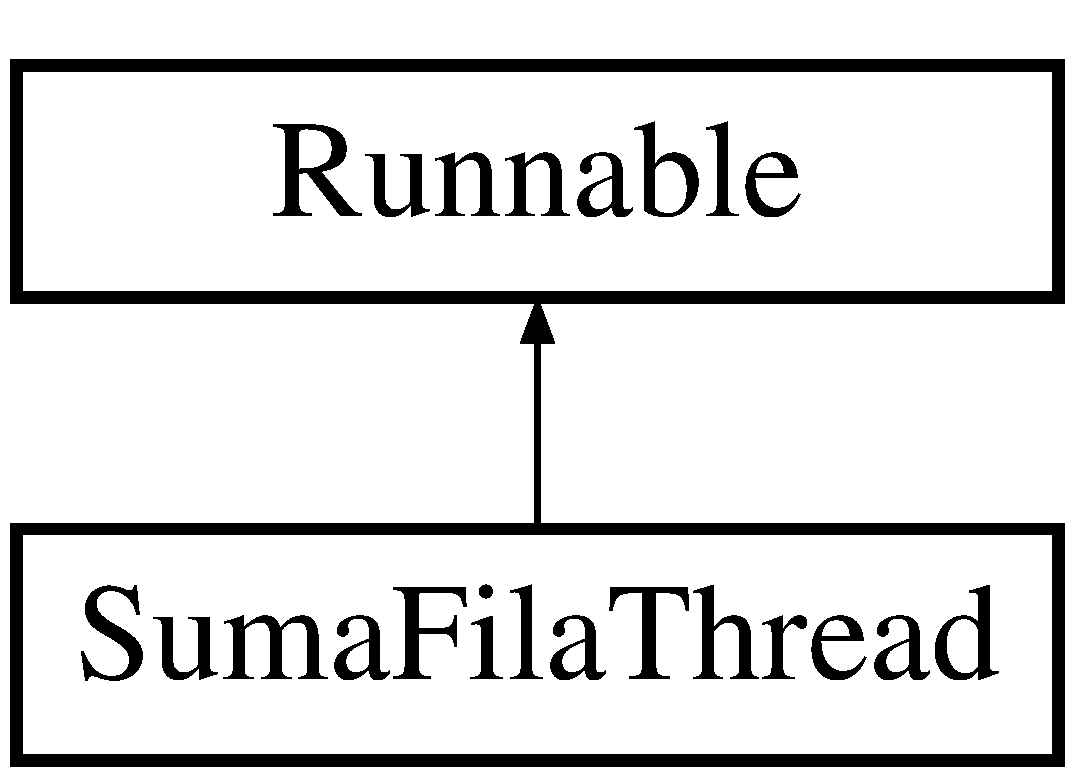
\includegraphics[height=2.000000cm]{classSumaFilaThread}
\end{center}
\end{figure}
\subsection*{Public Member Functions}
\begin{DoxyCompactItemize}
\item 
\hyperlink{classSumaFilaThread_a08b98e8d93693ed9f256529ab12af18f}{Suma\-Fila\-Thread} (int\mbox{[}$\,$\mbox{]} fila1, int\mbox{[}$\,$\mbox{]} fila2)
\item 
void \hyperlink{classSumaFilaThread_ad8fa946cd44e708f69cd98b3ec4c824e}{run} ()
\begin{DoxyCompactList}\small\item\em Realiza la suma de una fila de dos matrices y guarda el resultado. \end{DoxyCompactList}\item 
int\mbox{[}$\,$\mbox{]} \hyperlink{classSumaFilaThread_a6a2181a1a49bd2ef1169e3467b670e9f}{get\-Resultado} ()
\begin{DoxyCompactList}\small\item\em Devuelve el resultado de la suma realizada en el método \hyperlink{classSumaFilaThread_ad8fa946cd44e708f69cd98b3ec4c824e}{run()} \end{DoxyCompactList}\end{DoxyCompactItemize}


\subsection{Detailed Description}
Clase que se encarga de sumar una fila de dos matrices distintas. 

Cada objeto de esta clase se ejecuta en un único hilo. \begin{DoxyAuthor}{Author}
Martín y Víctor. 
\end{DoxyAuthor}


\subsection{Constructor \& Destructor Documentation}
\hypertarget{classSumaFilaThread_a08b98e8d93693ed9f256529ab12af18f}{\index{Suma\-Fila\-Thread@{Suma\-Fila\-Thread}!Suma\-Fila\-Thread@{Suma\-Fila\-Thread}}
\index{Suma\-Fila\-Thread@{Suma\-Fila\-Thread}!SumaFilaThread@{Suma\-Fila\-Thread}}
\subsubsection[{Suma\-Fila\-Thread}]{\setlength{\rightskip}{0pt plus 5cm}Suma\-Fila\-Thread.\-Suma\-Fila\-Thread (
\begin{DoxyParamCaption}
\item[{int\mbox{[}$\,$\mbox{]}}]{fila1, }
\item[{int\mbox{[}$\,$\mbox{]}}]{fila2}
\end{DoxyParamCaption}
)}}\label{classSumaFilaThread_a08b98e8d93693ed9f256529ab12af18f}


\subsection{Member Function Documentation}
\hypertarget{classSumaFilaThread_a6a2181a1a49bd2ef1169e3467b670e9f}{\index{Suma\-Fila\-Thread@{Suma\-Fila\-Thread}!get\-Resultado@{get\-Resultado}}
\index{get\-Resultado@{get\-Resultado}!SumaFilaThread@{Suma\-Fila\-Thread}}
\subsubsection[{get\-Resultado}]{\setlength{\rightskip}{0pt plus 5cm}int \mbox{[}$\,$\mbox{]} Suma\-Fila\-Thread.\-get\-Resultado (
\begin{DoxyParamCaption}
{}
\end{DoxyParamCaption}
)}}\label{classSumaFilaThread_a6a2181a1a49bd2ef1169e3467b670e9f}


Devuelve el resultado de la suma realizada en el método \hyperlink{classSumaFilaThread_ad8fa946cd44e708f69cd98b3ec4c824e}{run()} 

\begin{DoxyReturn}{Returns}
La fila resultado 
\end{DoxyReturn}
\hypertarget{classSumaFilaThread_ad8fa946cd44e708f69cd98b3ec4c824e}{\index{Suma\-Fila\-Thread@{Suma\-Fila\-Thread}!run@{run}}
\index{run@{run}!SumaFilaThread@{Suma\-Fila\-Thread}}
\subsubsection[{run}]{\setlength{\rightskip}{0pt plus 5cm}void Suma\-Fila\-Thread.\-run (
\begin{DoxyParamCaption}
{}
\end{DoxyParamCaption}
)}}\label{classSumaFilaThread_ad8fa946cd44e708f69cd98b3ec4c824e}


Realiza la suma de una fila de dos matrices y guarda el resultado. 



The documentation for this class was generated from the following file\-:\begin{DoxyCompactItemize}
\item 
src/\hyperlink{SumaFilaThread_8java}{Suma\-Fila\-Thread.\-java}\end{DoxyCompactItemize}

\hypertarget{interfaceSumaMatrices}{\section{Suma\-Matrices Interface Reference}
\label{interfaceSumaMatrices}\index{Suma\-Matrices@{Suma\-Matrices}}
}


Interfaz que define los métodos de las clases que implementen la suma de dos matrices.  


Inheritance diagram for Suma\-Matrices\-:\begin{figure}[H]
\begin{center}
\leavevmode
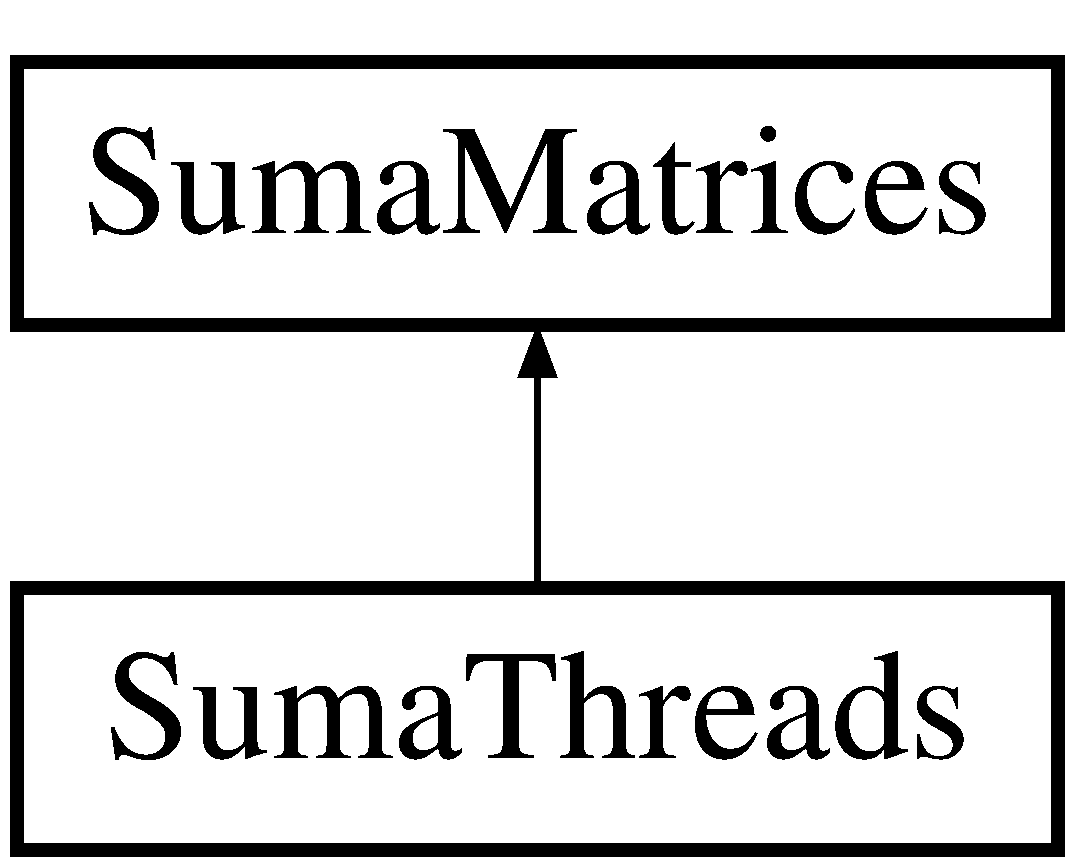
\includegraphics[height=2.000000cm]{interfaceSumaMatrices}
\end{center}
\end{figure}
\subsection*{Public Member Functions}
\begin{DoxyCompactItemize}
\item 
\hyperlink{classMatriz}{Matriz} \hyperlink{interfaceSumaMatrices_aaa4f45720c4f880570897a307d78c60d}{get\-Suma} (\hyperlink{classMatriz}{Matriz} m1, \hyperlink{classMatriz}{Matriz} m2)  throws Exception
\begin{DoxyCompactList}\small\item\em Obtiene la matriz que es suma de dos matrices. \end{DoxyCompactList}\end{DoxyCompactItemize}


\subsection{Detailed Description}
Interfaz que define los métodos de las clases que implementen la suma de dos matrices. 

\begin{DoxyAuthor}{Author}
Martín y Víctor 
\end{DoxyAuthor}


\subsection{Member Function Documentation}
\hypertarget{interfaceSumaMatrices_aaa4f45720c4f880570897a307d78c60d}{\index{Suma\-Matrices@{Suma\-Matrices}!get\-Suma@{get\-Suma}}
\index{get\-Suma@{get\-Suma}!SumaMatrices@{Suma\-Matrices}}
\subsubsection[{get\-Suma}]{\setlength{\rightskip}{0pt plus 5cm}{\bf Matriz} Suma\-Matrices.\-get\-Suma (
\begin{DoxyParamCaption}
\item[{{\bf Matriz}}]{m1, }
\item[{{\bf Matriz}}]{m2}
\end{DoxyParamCaption}
) throws Exception}}\label{interfaceSumaMatrices_aaa4f45720c4f880570897a307d78c60d}


Obtiene la matriz que es suma de dos matrices. 


\begin{DoxyParams}{Parameters}
{\em m1} & La primera matriz \\
\hline
{\em m2} & La segunda matriz \\
\hline
\end{DoxyParams}
\begin{DoxyReturn}{Returns}
La matriz resultante 
\end{DoxyReturn}

\begin{DoxyExceptions}{Exceptions}
{\em Exception} & que puede lanzar si las matrices son de distinto tamaño \\
\hline
\end{DoxyExceptions}


Implemented in \hyperlink{classSumaThreads_ac799c145a2711fff3ac9b348c8afd881}{Suma\-Threads}.



The documentation for this interface was generated from the following file\-:\begin{DoxyCompactItemize}
\item 
src/\hyperlink{SumaMatrices_8java}{Suma\-Matrices.\-java}\end{DoxyCompactItemize}

\hypertarget{classSumaThreads}{\section{Suma\-Threads Class Reference}
\label{classSumaThreads}\index{Suma\-Threads@{Suma\-Threads}}
}


Clase que implementa la suma de dos matrices utilizando hilos.  


Inheritance diagram for Suma\-Threads\-:\begin{figure}[H]
\begin{center}
\leavevmode
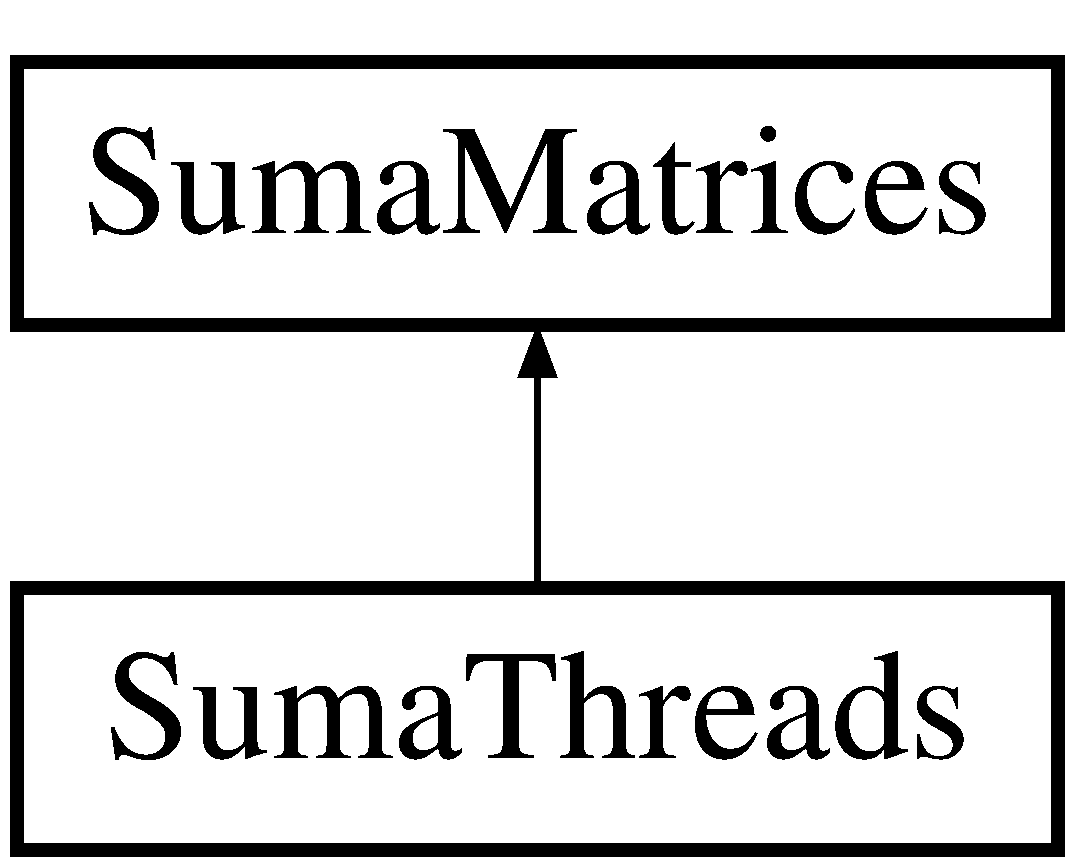
\includegraphics[height=2.000000cm]{classSumaThreads}
\end{center}
\end{figure}
\subsection*{Public Member Functions}
\begin{DoxyCompactItemize}
\item 
\hyperlink{classSumaThreads_a916580477ee278dc5785b878f0be789a}{Suma\-Threads} (int n\-Threads)  throws Exception 
\begin{DoxyCompactList}\small\item\em Constructor que recibe el número hilos. \end{DoxyCompactList}\item 
\hyperlink{classMatriz}{Matriz} \hyperlink{classSumaThreads_ac799c145a2711fff3ac9b348c8afd881}{get\-Suma} (\hyperlink{classMatriz}{Matriz} m1, \hyperlink{classMatriz}{Matriz} m2)  throws Exception 
\begin{DoxyCompactList}\small\item\em Obtiene la matriz que es suma de dos matrices. \end{DoxyCompactList}\end{DoxyCompactItemize}


\subsection{Detailed Description}
Clase que implementa la suma de dos matrices utilizando hilos. 

\begin{DoxyAuthor}{Author}
Víctor y Martín 
\end{DoxyAuthor}


\subsection{Constructor \& Destructor Documentation}
\hypertarget{classSumaThreads_a916580477ee278dc5785b878f0be789a}{\index{Suma\-Threads@{Suma\-Threads}!Suma\-Threads@{Suma\-Threads}}
\index{Suma\-Threads@{Suma\-Threads}!SumaThreads@{Suma\-Threads}}
\subsubsection[{Suma\-Threads}]{\setlength{\rightskip}{0pt plus 5cm}Suma\-Threads.\-Suma\-Threads (
\begin{DoxyParamCaption}
\item[{int}]{n\-Threads}
\end{DoxyParamCaption}
) throws Exception}}\label{classSumaThreads_a916580477ee278dc5785b878f0be789a}


Constructor que recibe el número hilos. 


\begin{DoxyParams}{Parameters}
{\em n\-Threads} & Número de hilos para resolver la suma \\
\hline
\end{DoxyParams}

\begin{DoxyExceptions}{Exceptions}
{\em Exception} & que se produce cuando el número hilos es negativo o 0 \\
\hline
\end{DoxyExceptions}


\subsection{Member Function Documentation}
\hypertarget{classSumaThreads_ac799c145a2711fff3ac9b348c8afd881}{\index{Suma\-Threads@{Suma\-Threads}!get\-Suma@{get\-Suma}}
\index{get\-Suma@{get\-Suma}!SumaThreads@{Suma\-Threads}}
\subsubsection[{get\-Suma}]{\setlength{\rightskip}{0pt plus 5cm}{\bf Matriz} Suma\-Threads.\-get\-Suma (
\begin{DoxyParamCaption}
\item[{{\bf Matriz}}]{m1, }
\item[{{\bf Matriz}}]{m2}
\end{DoxyParamCaption}
) throws Exception}}\label{classSumaThreads_ac799c145a2711fff3ac9b348c8afd881}


Obtiene la matriz que es suma de dos matrices. 


\begin{DoxyParams}{Parameters}
{\em m1} & La primera matriz \\
\hline
{\em m2} & La segunda matriz \\
\hline
\end{DoxyParams}
\begin{DoxyReturn}{Returns}
La matriz resultante 
\end{DoxyReturn}

\begin{DoxyExceptions}{Exceptions}
{\em Exception} & que puede lanzar si las matrices son de distinto tamaño \\
\hline
\end{DoxyExceptions}


Implements \hyperlink{interfaceSumaMatrices_aaa4f45720c4f880570897a307d78c60d}{Suma\-Matrices}.



The documentation for this class was generated from the following file\-:\begin{DoxyCompactItemize}
\item 
src/\hyperlink{SumaThreads_8java}{Suma\-Threads.\-java}\end{DoxyCompactItemize}

\chapter{File Documentation}
\hypertarget{Actividad2_8java}{\section{src/\-Actividad2.java File Reference}
\label{Actividad2_8java}\index{src/\-Actividad2.\-java@{src/\-Actividad2.\-java}}
}
\subsection*{Classes}
\begin{DoxyCompactItemize}
\item 
class \hyperlink{classActividad2}{Actividad2}
\begin{DoxyCompactList}\small\item\em Clase principal que muestra el resultado de la actividad 2. \end{DoxyCompactList}\end{DoxyCompactItemize}

\hypertarget{Matriz_8java}{\section{src/\-Matriz.java File Reference}
\label{Matriz_8java}\index{src/\-Matriz.\-java@{src/\-Matriz.\-java}}
}
\subsection*{Classes}
\begin{DoxyCompactItemize}
\item 
class \hyperlink{classMatriz}{Matriz}
\begin{DoxyCompactList}\small\item\em Clase que implementa los métodos necesarios para trabajar con una matriz cuadrada. \end{DoxyCompactList}\end{DoxyCompactItemize}

\hypertarget{SumaFilaThread_8java}{\section{src/\-Suma\-Fila\-Thread.java File Reference}
\label{SumaFilaThread_8java}\index{src/\-Suma\-Fila\-Thread.\-java@{src/\-Suma\-Fila\-Thread.\-java}}
}
\subsection*{Classes}
\begin{DoxyCompactItemize}
\item 
class \hyperlink{classSumaFilaThread}{Suma\-Fila\-Thread}
\begin{DoxyCompactList}\small\item\em Clase que se encarga de sumar una fila de dos matrices distintas. \end{DoxyCompactList}\end{DoxyCompactItemize}

\hypertarget{SumaMatrices_8java}{\section{src/\-Suma\-Matrices.java File Reference}
\label{SumaMatrices_8java}\index{src/\-Suma\-Matrices.\-java@{src/\-Suma\-Matrices.\-java}}
}
\subsection*{Classes}
\begin{DoxyCompactItemize}
\item 
interface \hyperlink{interfaceSumaMatrices}{Suma\-Matrices}
\begin{DoxyCompactList}\small\item\em Interfaz que define los métodos de las clases que implementen la suma de dos matrices. \end{DoxyCompactList}\end{DoxyCompactItemize}

\hypertarget{SumaThreads_8java}{\section{src/\-Suma\-Threads.java File Reference}
\label{SumaThreads_8java}\index{src/\-Suma\-Threads.\-java@{src/\-Suma\-Threads.\-java}}
}
\subsection*{Classes}
\begin{DoxyCompactItemize}
\item 
class \hyperlink{classSumaThreads}{Suma\-Threads}
\begin{DoxyCompactList}\small\item\em Clase que implementa la suma de dos matrices utilizando hilos. \end{DoxyCompactList}\end{DoxyCompactItemize}

%--- End generated contents ---

% Index
\newpage
\phantomsection
\addcontentsline{toc}{chapter}{Index}
\printindex

\end{document}
